\section{第十一章\quad 制冷循环}

\pt{逆向循环}：制冷循环和热泵循环均消耗外界功，把热量从低温对象转移到高温环境或供热对象。若无功输入，热量从低温传到高温会使孤立系 $\Delta S_{\mathrm{iso}}<0$，违背第二定律；实际必须满足 $\Delta S_{\mathrm{iso}}\ge 0$。

\pt{制冷系数}：$\varepsilon=\frac{q_c}{w_{\mathrm{net}}}=\frac{q_c}{q_0-q_c}$，$q_c$ 为从低温对象吸收的制冷量，$q_0$ 为向高温环境放热量。卡诺制冷循环 $\varepsilon_c=\frac{T_c}{T_0-T_c}$，温度必须用热力学温度。温差越小，理论 $\varepsilon_c$ 越大。

\pt{工程单位}：COP 即制冷装置工作性能系数；普通制冷常 $\varepsilon>1$，深冷常 $\varepsilon<1$。$1$ 冷吨约 $3.86\,\mathrm{kJ/s}$，美国制约 $3.517\,\mathrm{kJ/s}$。

\pt{热泵供热系数}：高温端供热量 $q_h=q_c+w_{\mathrm{net}}$，$\varepsilon_h=\frac{q_h}{w_{\mathrm{net}}}=\frac{q_c+w_{\mathrm{net}}}{w_{\mathrm{net}}}=1+\varepsilon>1$。热泵关注高温端放热，制冷机关注低温端吸热。

\divider

\pt{压缩空气制冷循环（逆布雷顿）}

\begin{center}
    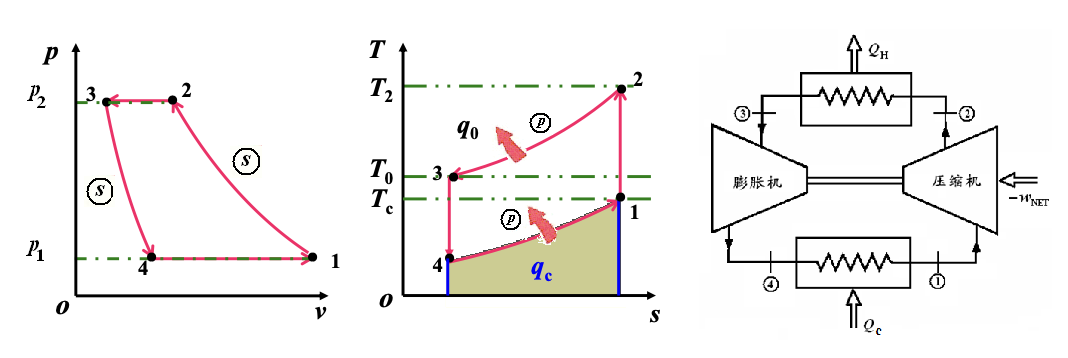
\includegraphics[width=\linewidth]{figures/11制冷循环.png}
\end{center}

$1$-$2$ 压缩机等熵压缩，$2$-$3$ 冷却器定压放热，$3$-$4$ 膨胀机等熵膨胀，$4$-$1$ 冷端定压吸热。

\pt{制冷系数}在工程上也称制冷装置的工作性能系数，即 $\mathrm{COP}$。$\varepsilon=\frac{q_\mathrm{c}}{q_0-q_\mathrm{c}}$ ，若为卡诺循环 $\varepsilon_\mathrm{c}=\frac{T_\mathrm{c}}{T_0-T_\mathrm{c}}$

深冷装置通常 $\varepsilon<1$，普通制冷装置通常 $\varepsilon>1$。

\pt{冷吨}定义：$1000\ \mathrm{kg}$、$0^\circ\mathrm{C}$ 饱和水在 $24\ \mathrm{h}$ 内冻结成 $0^\circ\mathrm{C}$ 冰所需的制冷量。$1$ 冷吨 $=3.86\ \mathrm{kJ/s}$；美国制 $1$ 冷吨 $=3.517\ \mathrm{kJ/s}$

\pt{能量关系}：制冷量 $q_c=h_1-h_4$，$q_0=h_2-h_3$，$w_{\mathrm{net}}=(h_2-h_1)-(h_3-h_4)$，$\varepsilon=\frac{h_1-h_4}{(h_2-h_1)-(h_3-h_4)}$。

\pt{理想气体定比热}情况：设 $\pi=\frac{p_2}{p_1}$，则 $T_2=T_1\pi^{(\kappa-1)/\kappa}$，$T_3=T_4\pi^{(\kappa-1)/\kappa}$，$\varepsilon=\frac{1}{\pi^{(\kappa-1)/\kappa}-1}=\frac{T_1}{T_2-T_1}$。$\pi\downarrow$ 时 $\varepsilon\uparrow$，但循环制冷量 $q_c$ 可能下降。

\newcolumn

\begin{center}
    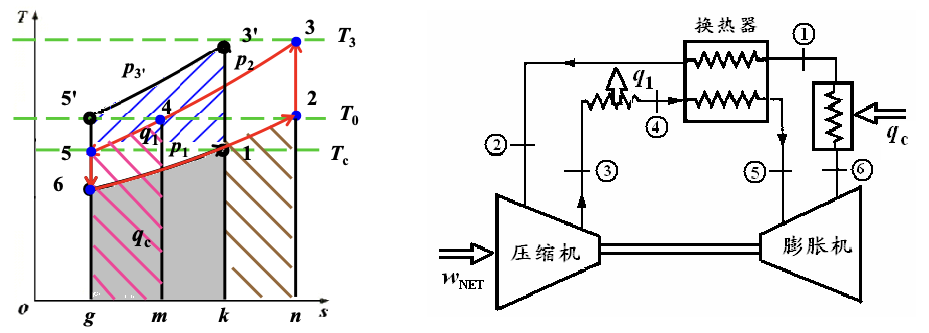
\includegraphics[width=0.8\linewidth]{figures/11回热式压缩空气制冷循环.png}
\end{center}

自冷库出来的空气（温度为 $T_1$，即低温热源温度 $T_{\mathrm{c}}$），首先进入回热器升温到高温热源的温度 $T_2$（通常为环境温度 $T_0$），接着进入叶轮式压气机进行压缩，升温、升压到 $T_3$、$p_3$，再进入冷却器，实现定压放热，降温至 $T_4$（理论上可达高温热源温度 $T_2$），随后进入回热器进一步定压降温至 $T_5$（即低温热源温度 $T_{\mathrm{c}}$），再进入叶轮式膨胀机实现定熵膨胀过程，降压、降温至 $T_6$、$p_6$，最后进入冷库实现定压吸热，升温到 $T_1$，完成循环。

\begin{itemize}
    \item 回热前：$q_1=\text{面积 }3'5'gk3'$，$q_\mathrm{c}=\text{面积 }16gk1$。
    \item 回热后：$\text{面积 }21kn2=\text{面积 }45gm4$，表示回热器内冷热流体换热量相等。
    \item 回热后：$q_\mathrm{c}=\text{面积 }16gk1$，$q_1=\text{面积 }34mn3=\text{面积 }3'5'gk3'$。
    \item 因此回热前后 $q_1$ 相等、$q_\mathrm{c}$ 相等，$w_\mathrm{net}$ 也相等，所以 $\varepsilon$ 相等。
    \item 但回热后压力比降低，课件给出 $\pi_1={p_3}/{p_2}<\pi_2={p_{3'}}/{p_1}$。
    \item 结论：回热不一定提高该理想比较下的 $\varepsilon$，但能在相同制冷量和相同净功条件下降低所需压力比，使装置更易实现。
\end{itemize}

\divider

\noindent
\begin{minipage}
    [t]{0.64\linewidth}
    \vspace{0pt}
    \raggedright
    \pt{压缩蒸气制冷循环}：
    主要设备包括压缩机、冷凝器、节流阀或毛细管、蒸发器。

    $1$-$2$ 压缩机压缩；$2$-$3$-$4$ 冷凝器放热并冷凝；$4$-$5$ 节流阀降压，近似等焓 $h_5=h_4$；$5$-$1$ 蒸发器吸热汽化。相变使单位质量制冷量大，工程制冷常用。
    \par\vspace{1pt}
    \pt{制冷系数}：$q_c=h_1-h_5=h_1-h_4$，$q_0=h_2-h_4$，$w_{\mathrm{net}}=h_2-h_1$，$\varepsilon=\frac{h_1-h_4}{h_2-h_1}$。不能用 $\frac{T_1-T_4}{T_2-T_1}$ 代替焓差。
\end{minipage}
\hfill
\begin{minipage}
    [t]{0.35\linewidth}
    \vspace{0pt}
    \centering
    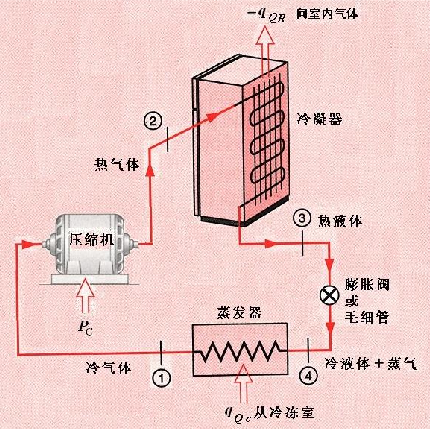
\includegraphics[width=\linewidth]{figures/11压缩制冷设备.png}
\end{minipage}

\divider

\noindent
\begin{minipage}
    [t]{0.35\linewidth}
    \vspace{0pt}
    \raggedright
    \pt{$\log p$-$h$ 图}：横坐标为焓 $h$，纵坐标为 $\log p$，适合压缩蒸气制冷循环查图计算。核心用途是确定各状态点后，直接用焓差求制冷量、压缩功、放热量和制冷系数。

    \begin{itemize}
        \item 定压过程在 $\log p$-$h$ 图上近似为水平线。
        \item 蒸发器过程 $5$-$1$ 位于低压线，即蒸发器压力线上。
        \item 冷凝器过程 $2$-$4$ 位于高压线，即冷凝器压力线上。
        \item 节流过程 $4$-$5$ 近似等焓，故 $h_5=h_4$，在图上近似为竖直线。
    \end{itemize}


\end{minipage}
\hfill
\begin{minipage}
    [t]{0.64\linewidth}
    \vspace{0pt}
    \centering
    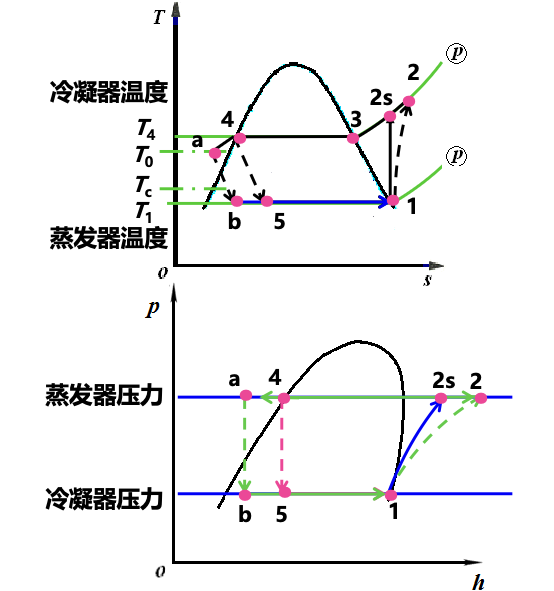
\includegraphics[width=\linewidth]{figures/11logpht.png}
\end{minipage}

\begin{itemize}
    \item 压缩过程 $1$-$2s$ 表示理想等熵压缩，$1$-$2$ 表示实际压缩。
\end{itemize}

\pt{循环计算}：
\begin{itemize}
    \item 制冷量：$q_c=h_1-h_5=h_1-h_4$。
    \item 冷凝器放热量：$q_1=h_2-h_4$。
    \item 压缩机耗功：$w_{\mathrm{net}}=h_2-h_1$。
    \item 制冷系数：$\varepsilon=\frac{q_c}{w_{\mathrm{net}}}=\frac{h_1-h_4}{h_2-h_1}$。
    \item 过冷循环：$\varepsilon_{\mathrm{SC}}=\frac{h_1-h_b}{h_2-h_1}$。
\end{itemize}

\pt{液体过冷}：冷凝器出口由 $4$ 过冷到 $b$，节流后焓降低，$\varepsilon_{\mathrm{SC}}=\frac{h_1-h_b}{h_2-h_1}>\varepsilon$，单位质量制冷量增大。

\pt{提高压缩蒸气制冷系数}：降低冷凝温度、提高蒸发温度、减少不可逆压缩损失、采用液体过冷、减少节流损失。

\pt{制冷剂要求}：
\begin{itemize}
    \item \pt{热力性质}：对应制冷装置工作温度时，饱和压力应适中；汽化潜热应大，这样单位质量制冷量 $q_\mathrm{c}$ 较大；临界温度应高于环境温度，便于在环境温度附近冷凝；蒸气比体积应小，有利于减小压缩机体积流量和设备尺寸；导热系数应大，有利于换热器传热；蒸发压力不宜低于环境压力，避免系统在负压下运行并吸入空气；三相点应低于制冷循环下限温度，避免工作范围内出现固化问题；在 $T$-$s$ 图上，上、下界限线应较陡峭，使冷凝更接近定温放热，并减少节流引起的制冷能力损失。
    \item \pt{其他性质}：对环境友善；安全无毒；溶油性好；化学稳定性好。
\end{itemize}

\noindent
\begin{minipage}
    [t]{0.35\linewidth}
    \vspace{0pt}
    \raggedright
    \pt{热泵循环}：热泵循环与制冷循环使用相似的逆向循环装置

    \pt{供热系数}：$\varepsilon'=\frac{w_{\mathrm{net}}+q_2}{w_{\mathrm{net}}}=1+\frac{q_2}{w_{\mathrm{net}}}>1$
\end{minipage}
\hfill
\begin{minipage}
    [t]{0.64\linewidth}
    \vspace{0pt}
    \centering
    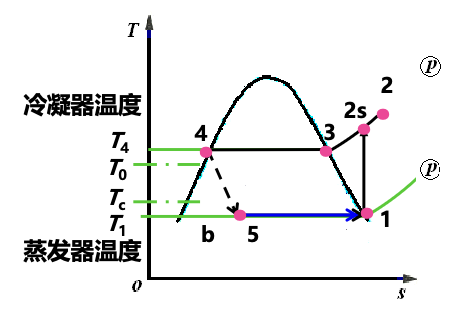
\includegraphics[width=\linewidth]{figures/11热泵循环.png}
\end{minipage}

\pt{供暖例子}：
\begin{itemize}
    \item 工业锅炉效率为 $\eta_{\mathrm{B}}=0.7$，则 $Q=Q_{\mathrm{a}}\eta_{\mathrm{B}}=0.7Q_{\mathrm{a}}$。
    \item 电厂热效率为 $\eta_{\mathrm{t}}=0.35$，热泵供暖系数为 $\varepsilon'=3$。
    \item 若用一次能源 $Q_{\mathrm{a}}$ 发电后驱动热泵，则供热量为 $Q=Q_{\mathrm{a}}\eta_{\mathrm{t}}\varepsilon'=1.05Q_{\mathrm{a}}$。
    \item 这个例子说明，在给定参数下，热泵供暖可比直接锅炉供暖获得更高的有效供热量。
\end{itemize}

\begin{center}
    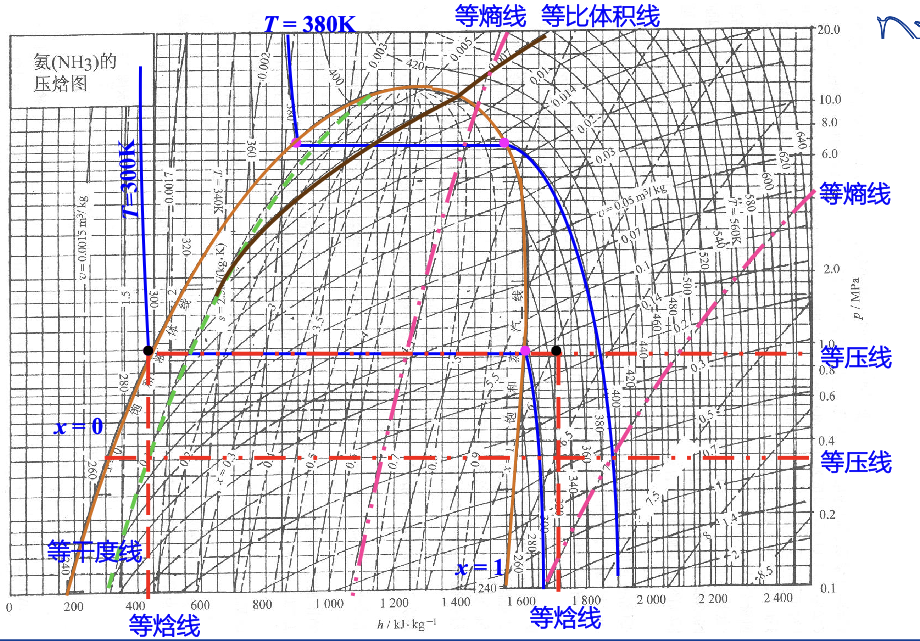
\includegraphics[width=\linewidth]{figures/11氨焓压图.png}
\end{center}

孩子们这是啥
\divider
